\documentclass{ximera}
\input{../preamble}

\title[Dig-In:]{Consumers' and producers' surplus}

\begin{document}
\begin{abstract}
  \end{abstract}
\maketitle

In this section, we will assume that the market is at equilibrium. This means that we are considering what happens when the quantity 
demanded $q_{0}$ is the same as the quantity supplied, while simultaneously the price paid $p_{0}$ is the same as the
selling price. 

In context, if $D(q)$ is the demand curve and $S(q)$ is the supply curve, then the point $(q_{0},p_{0})$ is the intersection of the 
curves $D(q)$ and $S(q)$. 

At the equilibrium price, there are consumers who would be willing to purchase some units at a price higher than $p_{0}$. 
As such, consumers receive a benefit in the form of paying less than they otherwise might have. This benefit 
to the consumers is called the {\bf consumers' surplus}. The total benefit is given by the area over the 
interval $[0,q_{0}]$ and bounded by the demand curve $D(q)$ and the line $p=p_{0}$.


\begin{image}
\begin{tikzpicture}
	\begin{axis}[
            ticks=none, domain=0:20, ymax=25,xmax=15,ymin=-2, xmin=-2,
            axis lines =center, xlabel=$q$, ylabel=$p$,
	   %xtick={0.5635,1},
            %xticklabels={$a$,$1$}, 
            every axis y label/.style={at=(current axis.above origin),anchor=south},
            every axis x label/.style={at=(current axis.right of origin),anchor=west},
            axis on top,
          ]
          %\addplot [draw=none,fill=fillp,domain=0:12] {2+0.0556*x^2} \closedcycle;
          \addplot [draw=none,fill=background,domain=0:12] {20-0.0694*x^2} \closedcycle;
          %\addplot [draw=none,fill=background,domain=0:12] {10} \closedcycle;
           \addplot [draw=none,fill=fillp,domain=0:12] {20-0.0694*x^2} \closedcycle;
          \addplot [draw=none,fill=fillp,domain=0:12] {10} \closedcycle;
          \addplot [draw=none,fill=background,domain=0:12] {10} \closedcycle;
          \addplot [draw=penColor,very thick] {20-0.0694*x^2};
          \addplot [draw=penColor2,very thick] {2+0.0556*x^2};
          \node at (axis cs:6,2) [penColor2] {$S(q)$};
          \node at (axis cs:1.25,22) [penColor] {$D(q)$};  
          \node at (axis cs:3,15) [penColor3] {CS};
           \node at (axis cs:12,-1) [penColor3] {$q_{0}$};
          \node at (axis cs:-0.75,10) [penColor3] {$p_{0}$};
          \addplot [textColor,dashed] plot coordinates {(12,0) (12,20)};
          \addplot [textColor,dashed] plot coordinates {(0,10) (30,10)};
          \addplot[color=penColor3,fill=penColor3,only marks,mark=*] coordinates{(12,10)};  %% closed hole 

        \end{axis}
\end{tikzpicture}
\end{image}

As the consumers' surplus is the area between two curves, it corresponds to an integral. In particular:
\begin{image}
  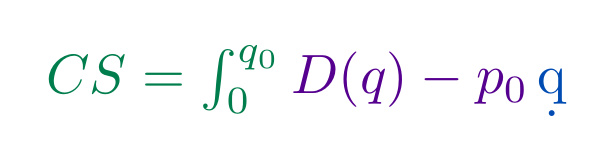
\begin{tikzpicture}[scale=2,every node/.style={transform shape}]
    \node at (0,0) {
      $\color{green!70!black!70!blue}CS=\int_{0}^{q_{0}}\color{purple!50!blue!90!black}{D(q)-p_{0}} \,\color{blue!70!green}{\d q}$
    };
  \end{tikzpicture}
\end{image}

There is a similar situation for producers. At the equilibrium price, the producer would be willing to sell some units at a price lower than $p_{0}$. 
As such, the producer receives a benefit in the form of receiving more revenue that the might otherwise would have. This benefit 
to the producers is called the {\bf producers' surplus}. The total benefit is given by the area over the 
interval $[0,q_{0}]$ and bounded by the supply curve $S(q)$ and the line $p=p_{0}$.




\begin{image}
\begin{tikzpicture}
	\begin{axis}[
            ticks=none, domain=0:20, ymax=25,xmax=15,ymin=-2, xmin=-2,
            axis lines =center, xlabel=$q$, ylabel=$p$,
	   %xtick={0.5635,1},
            %xticklabels={$a$,$1$}, 
            every axis y label/.style={at=(current axis.above origin),anchor=south},
            every axis x label/.style={at=(current axis.right of origin),anchor=west},
            axis on top,
          ]
          \addplot [draw=none,fill=fillp,domain=0:12] {2+0.0556*x^2} \closedcycle;
          %\addplot [draw=none,fill=background,domain=0:12] {20-0.0694*x^2} \closedcycle;
          \addplot [draw=none,fill=background,domain=0:12] {10} \closedcycle;
           %\addplot [draw=none,fill=fillp,domain=0:12] {20-0.0694*x^2} \closedcycle;
          \addplot [draw=none,fill=fillp,domain=0:12] {10} \closedcycle;
          \addplot [draw=none,fill=background,domain=0:12] {2+0.0556*x^2} \closedcycle;
          \addplot [draw=penColor,very thick] {20-0.0694*x^2};
          \addplot [draw=penColor2,very thick] {2+0.0556*x^2};
          \node at (axis cs:6,2) [penColor2] {$S(q)$};
          \node at (axis cs:1.25,22) [penColor] {$D(q)$};  
          \node at (axis cs:3,6) [penColor3] {PS};
          \node at (axis cs:12,-1) [penColor3] {$q_{0}$};
          \node at (axis cs:-0.75,10) [penColor3] {$p_{0}$};
          \addplot [textColor,dashed] plot coordinates {(12,0) (12,20)};
          \addplot [textColor,dashed] plot coordinates {(0,10) (30,10)};
          \addplot[color=penColor3,fill=penColor3,only marks,mark=*] coordinates{(12,10)};  %% closed hole 

        \end{axis}
\end{tikzpicture}
\end{image}

As the producers' surplus is the area between two curves, it corresponds to an integral. In particular:

\begin{image}
  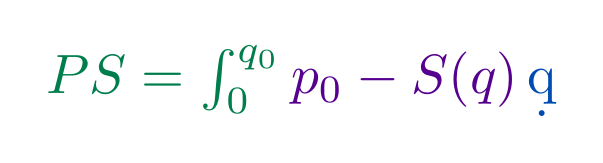
\begin{tikzpicture}[scale=2,every node/.style={transform shape}]
    \node at (0,0) {
      $\color{green!70!black!70!blue}PS=\int_{0}^{q_{0}}\color{purple!50!blue!90!black}{p_{0}-S(q)} \,\color{blue!70!green}{\d q}$
    };
  \end{tikzpicture}
\end{image}

A good way to remember which area corresponds to which surplus is that consumers {\bf demand} and producers {\bf supply}. 
This means that the area corresponding to the consumers' surplus is the one bounded by the demand function and the area 
corresponding to the producers' surplus is the one bounded by the supply function.

\begin{example}
  Suppose that the demand function for a product is:
  $$D(q) = 30-2q$$
  and the supply function for this product is 
  $$S(q) = 12+q$$
  Find the consumers' surplus and producers' surplus at market equilibrium
\begin{image}
\begin{tikzpicture}
	\begin{axis}[
            ticks=none, domain=0:10, ymax=35,xmax=10,ymin=-2, xmin=-2,
            axis lines =center, xlabel=$q$, ylabel=$p$,
	   %xtick={0.5635,1},
            %xticklabels={$a$,$1$}, 
            every axis y label/.style={at=(current axis.above origin),anchor=south},
            every axis x label/.style={at=(current axis.right of origin),anchor=west},
            axis on top,
          ]
          \addplot [draw=none,fill=fillp!50!white,domain=0:12] {12+x} \closedcycle;
         \addplot [draw=none,fill=background,domain=0:12] {30-2*x} \closedcycle;
          \addplot [draw=none,fillp!50!white=background,domain=0:12] {18} \closedcycle;
         \addplot [draw=none,fill=fillp!50!white,domain=0:12] {30-2*x} \closedcycle;
          \addplot [draw=none,fill=fillp,domain=0:10] {18} \closedcycle;
          \addplot [draw=none,fill=background,domain=0:12] {12+x} \closedcycle;
          \addplot [draw=penColor,very thick] {30-2*x};
          \addplot [draw=penColor2,very thick] {12+x};
          \node at (axis cs:2,12) [penColor2] {$S(q)$};
          \node at (axis cs:2,29) [penColor] {$D(q)$};  
          \node at (axis cs:1,16) [penColor3] {PS};
         \node at (axis cs:1,25) [penColor3] {CS};
          \node at (axis cs:6,-1) [penColor3] {$q_{0}$};
          \node at (axis cs:-0.75,18) [penColor3] {$p_{0}$};
          \addplot [textColor,dashed] plot coordinates {(6,0) (6,35)};
          \addplot [textColor,dashed] plot coordinates {(0,18) (10,18)};
          \addplot[color=penColor3,fill=penColor3,only marks,mark=*] coordinates{(6,18)};  %% closed hole 

        \end{axis}
\end{tikzpicture}
\end{image}




\begin{explanation}
First we need to find the market equillibrium. We do this by equating the demand and supply functions
\begin{align*}
  D(q) &= S(q) \\
  30-2q &= 12+q 
\end{align*} 
Then 
$$\answer[given]{18} = \answer[given]{3q}$$
So
$$q_{0}=\answer[given]{6}$$
Now that we know $q_{0}$ we can find $p_{0}$ using either the demand function or the supply function. We will
use the supply function:
\begin{align*}
  p_{0} &= S(q_{0}) \\
   	   &= 12+\answer[given]{6} \\
	   &= \answer[given]{18}
\end{align*}
Now we can proceed to find the surpluses. We will find the consumers' surplus first:
\[ 
CS = \int_{\answer[given]{0}}^{\answer[given]{6}} D(q) - \answer[given]{18} \d q = \answer[given]{36}
\]
\begin{hint}
\[
\int_0^6 (30-2q)-(18) \d q
\]
\begin{align*}
  &=\int_0^6 12-2q \d q \\
  &=\eval{12q-q^2}_0^6 \\
  &= (72-36)-(0) \\
  &=36
\end{align*}
\end{hint}
Next, we find the producers' surplus:
\[ 
PS = \int_{\answer[given]{0}}^{\answer[given]{6}}  \answer[given]{18}-S(q) \d q = \answer[given]{18}
\]
\begin{hint}
\[
\int_0^6 (18)-(12+q) \d q
\]
\begin{align*}
  &=\int_0^6 6-q \d q \\
  &=\eval{6q-\frac{q^2}{2}}_0^6 \\
  &= (36-18)-(0) \\
  &=18
\end{align*}
\end{hint}
\end{explanation}
\end{example}
























\end{document}

